\documentclass{beamer}

\usepackage[utf8]{inputenc}
\usepackage{default}
\usepackage{graphicx}
\usepackage{bbding}
\usepackage{color}

% TODO Learn what this does
% source
% http://tex.stackexchange.com/questions/15952/layout-of-multiple-lines-footnotes
% this is a way to adjust foot note so it can be cutted into multiple lines
\makeatletter
\renewcommand\@makefntext[1]{\tiny\rightskip=25em\hskip0em\@makefnmark#1}
\makeatother

\makeatletter
\newcommand*{\rom}[1]{\expandafter\@slowromancap\romannumeral #1@}
\makeatother

% shows how to change default (blue) colours in the default beamer theme
% found here: http://joerglenhard.wordpress.com/tag/latex/
\definecolor{WaterlooRed}{RGB}{145,11,46}
\setbeamercolor{title}{fg=WaterlooRed}
\setbeamercolor{frametitle}{fg=WaterlooRed}
\setbeamercolor{structure}{fg=WaterlooRed}

% Added line numbers in footnote
% source: http://tex.stackexchange.com/questions/137022/how-to-insert-page-number-in-beamer-navigation-bars
\addtobeamertemplate{navigation symbols}{}{%
  \usebeamerfont{footline}%
  \usebeamercolor[fg]{footline}%
  \hspace{1em}%
  \insertframenumber%/\inserttotalframenumber
}
\setbeamercolor{footline}{fg=WaterlooRed}
% end of added line numbers in footnote



% adds logo in the footer
\logo{
\includegraphics[scale=.25]{img/csuow}}

\title[]{MicroFuge: A Middleware Approach to Providing Performance Isolation in Cloud Storage Systems}
\author[Akshay Singh, Xu Cui, Benjamin Cassell, Bernard Wong and Khuzaima Daudjee]{Akshay Singh,   \textcolor{WaterlooRed}{\textbf{Xu Cui}}, Benjamin Cassell, Bernard Wong and Khuzaima Daudjee}
\institute{
\includegraphics[scale=0.25]{img/UniversityOfWaterloo_logo_vert_rgb.png}}
\date{{\tiny\today}}


% my macros
\newcommand{\myv}{\vspace{3 mm}}

\begin{document}

\begin{frame}
  \titlepage
\end{frame}

\begin{frame}
  \frametitle{Storage Resources in Cloud Datacenters}
\vspace{-5 mm}
    \begin{itemize}
    \item Cloud computing allows sharing of resource at the cost of reduced isolation.
      \newline
    \item Storage systems are highly sensitive to performance interference.
      \newline
    \item \(\text{Lack of performance isolation} \rightarrow \text{Unpredictable latencies.}\)
    \end{itemize}
\end{frame}

\begin{frame}
  \frametitle{A Cloud Scenario}
  %% \vspace{5 mm}
  \begin{itemize}
  \item In worst case, a particular HTTP request may require 35 database
    lookups.${^{1}}$
    %% \footnote{Nathan Farrington and Alexey Andreyev, Facebook’s Data
      %% Center Network Architecture.}
    \begin{itemize}
      \myv
    \item  Response time can add up quickly.
    \end{itemize}
    \myv
  \item Amazon reported 100ms of latency cost them 1\% in sales.${^{2}}$
    \myv
  \item Google found an extra .5 seconds delay caused 20\% drop in search
    traffic.${^{2}}$
    %% \centering
    \myv
    \myv
    \myv
    \myv
  \item[--] \footnotesize{[1] Nathan Farrington and Alexey Andreyev, Facebook’s Data
    Center Network Architecture.}
  \item[--] \footnotesize{[2] Greg Lindem, Make Data Useful,
    \url{http://www.scribd.com/doc/4970486/Make-Data-Useful-by-Greg-Linden-Amazon-com}.}
  \end{itemize}
\end{frame}

\begin{frame}
  \frametitle{Performance Isolation}
  \begin{itemize}
  \item Clients want to have performance guarantees in the shared
    environment. \myv
  \item Possible solutions to performance isolation.
    \myv
    %% \vspace{-2.5 mm}
    \begin{itemize}
    \item Dedicated resources.
      \myv
    \item Meet clients' response time requirements in the shared environment.
      \myv
      \begin{itemize}
      \item We represent response time requirements with \textbf{request deadlines}.
      \end{itemize}
      \myv
    \item \(\text{Meeting request deadlines} \rightarrow \text{Performance isolation.}\)
    \end{itemize}
  \end{itemize}
\end{frame}

\begin{frame}
  \frametitle{MicroFuge}
  \begin{itemize}
  \item A distributed caching and scheduling middleware that provides
    performance isolation.
    \myv
    \begin{itemize}
    \item \textbf{Deadline Cache (DLC)}
      \myv
      \begin{itemize}
      \item Builds a performance model of the system.
        \myv
      \item Uses multiple LRU queues for deadline-aware eviction.
        \myv
      \end{itemize}
    \item \textbf{Deadline Scheduler (DLS)}
      \begin{itemize}
        \myv
      \item Performs intelligent replica selection.
        \myv
      \item Implements feedback-driven deadline-aware scheduling.
        \myv
        %% \item {\textcolor[gray]{0.5} {Optionally performs admission control.}}
      \item Optionally performs admission control.
      \end{itemize}
    \end{itemize}
    \myv
  \item Middleware: supports different cloud storage systems.
  \end{itemize}
\end{frame}

%% xcuiTODO: add the next slide to my latex sample/tutorial slides
%% \begin{frame}
  %% \frametitle{useful color text tutorial}
  %% \url{http://www-h.eng.cam.ac.uk/help/tpl/textprocessing/latex_advanced/colorandfonts.html}
  %% \\
  %% \myv
  %% \definecolor{gold}{rgb}{0.85,.66,0}
  %% This is in \textcolor{red}{red} and this box is \colorbox{gold}{gold}.
  %% Text color can be set using RGB values
  %% (\textcolor[rgb]{0,1,0}{like so}), or \textcolor[gray]{0.2}{shades}
  %% \textcolor[gray]{0.5}{of} \textcolor[gray]{0.8}{grey}.
%% \end{frame}

%% \begin{frame}
  %% \frametitle{MicroFuge Overview (1)}
  %% \vspace{-5 mm}
  %% \begin{center}
    %% 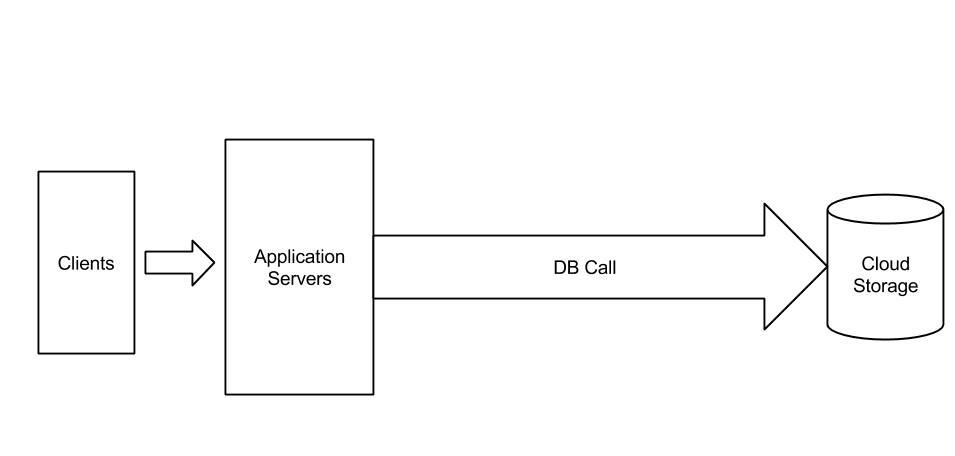
\includegraphics[scale=0.33]{img/MF_FULL_NEW_1.png}
    %% 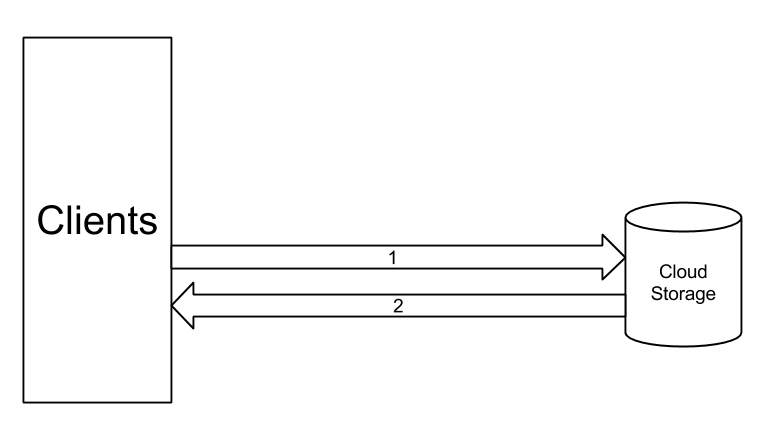
\includegraphics[scale=0.39]{img/MF_FULL_V8_1.png}
  %% \end{center}
%% \end{frame}

\begin{frame}
  \frametitle{MicroFuge Overview \rom{1}}
  %% \vspace{-5 mm}
  \begin{center}
    %% 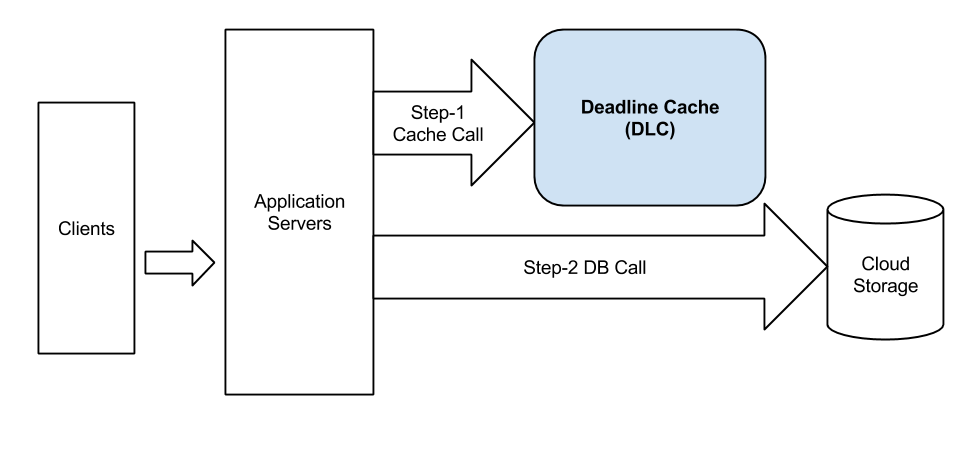
\includegraphics[scale=0.33]{img/MF_FULL_NEW_2.png}
    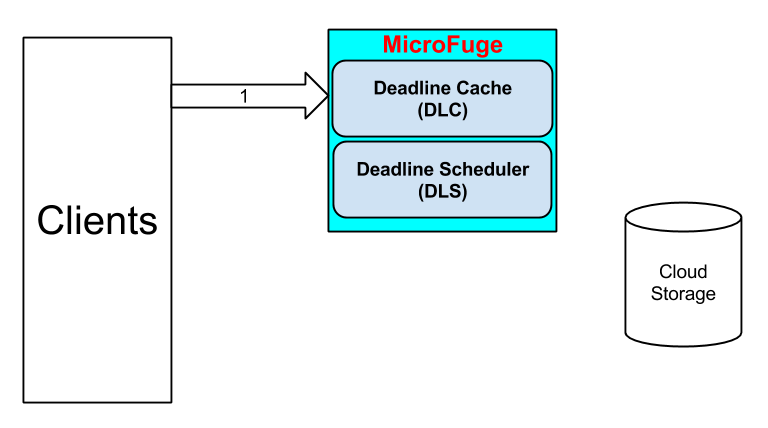
\includegraphics[scale=0.39]{img/MF_FULL_V8_2.png}
  \end{center}
\end{frame}

\begin{frame}
  \frametitle{MicroFuge Overview \rom{2}}
  %% \vspace{-5 mm}
  \begin{center}
    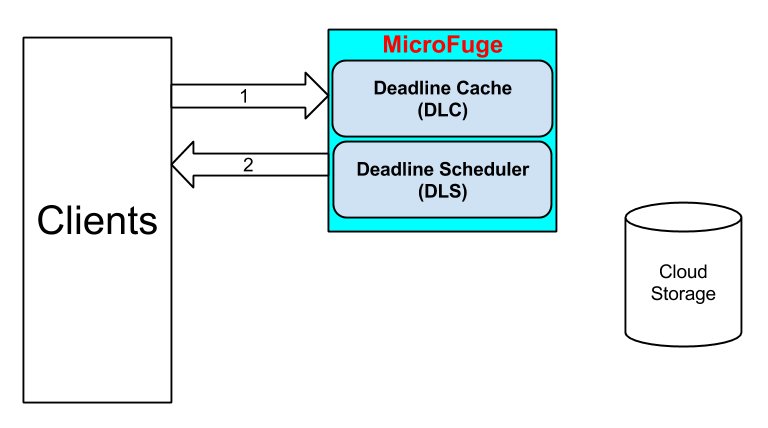
\includegraphics[scale=0.39]{img/MF_FULL_V8_3.png}
  \end{center}
\end{frame}

\begin{frame}
  \frametitle{MicroFuge Overview \rom{3}}
  %% \vspace{-5 mm}
  \begin{center}
    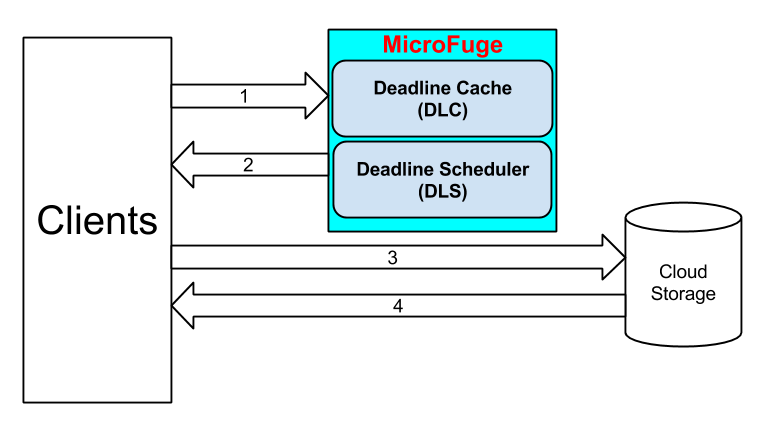
\includegraphics[scale=0.39]{img/MF_FULL_V8_4.png}
  \end{center}
\end{frame}

\begin{frame}
  \frametitle{Deadline Cache (DLC) - Components}
  \vspace{0.5 mm}
  \begin{figure}
    \begin{center}
      %% next line is the scale for screenshots taken at school
      %% \centerline{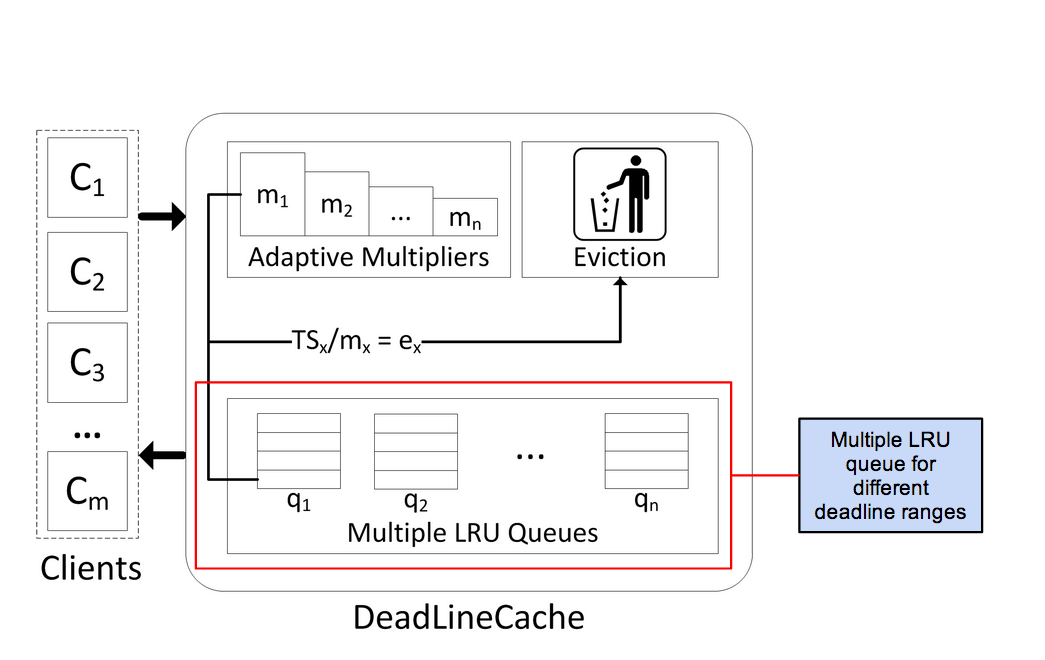
\includegraphics[scale=0.45]{img/DLC_ARC_1.png}}
      \centerline{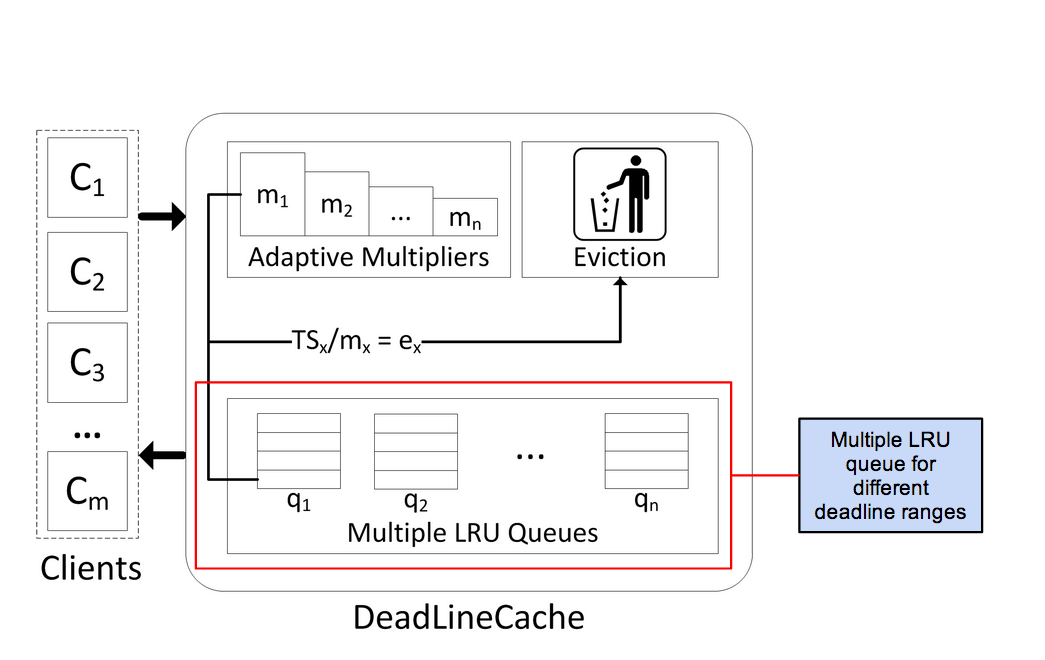
\includegraphics[scale=0.33]{img/DLC_ARC_1.png}}
    \end{center}
  \end{figure}
\end{frame}

\begin{frame}
  \frametitle{Deadline Cache (DLC) - Components}
  \begin{figure}
    \begin{center}
      %% next line is the scale for screenshots taken at school
      %% \centerline{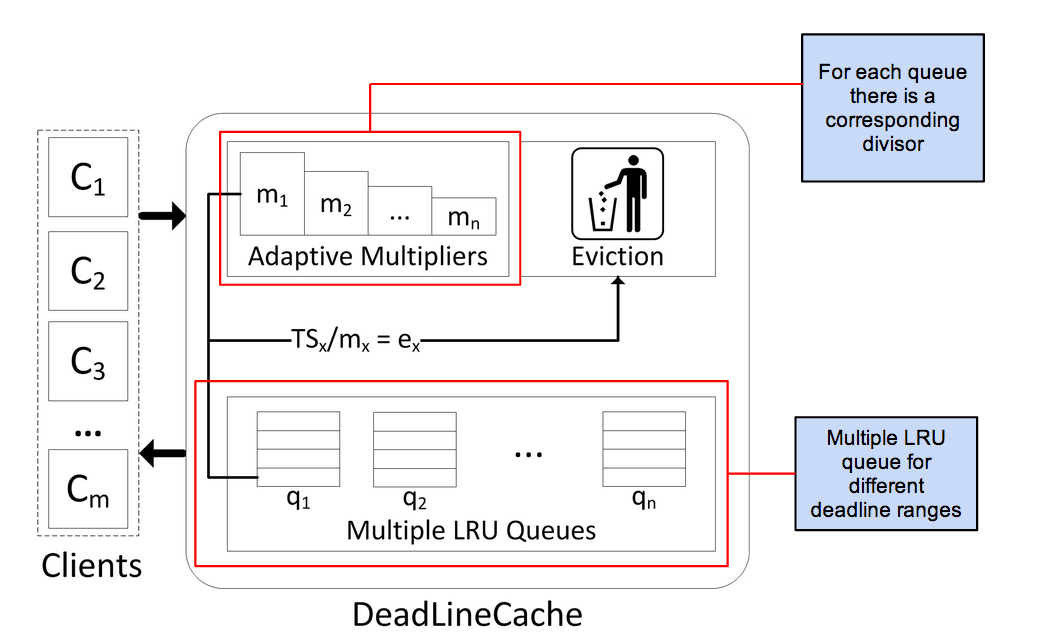
\includegraphics[scale=0.45]{img/DLC_ARC_2.png}}
      \centerline{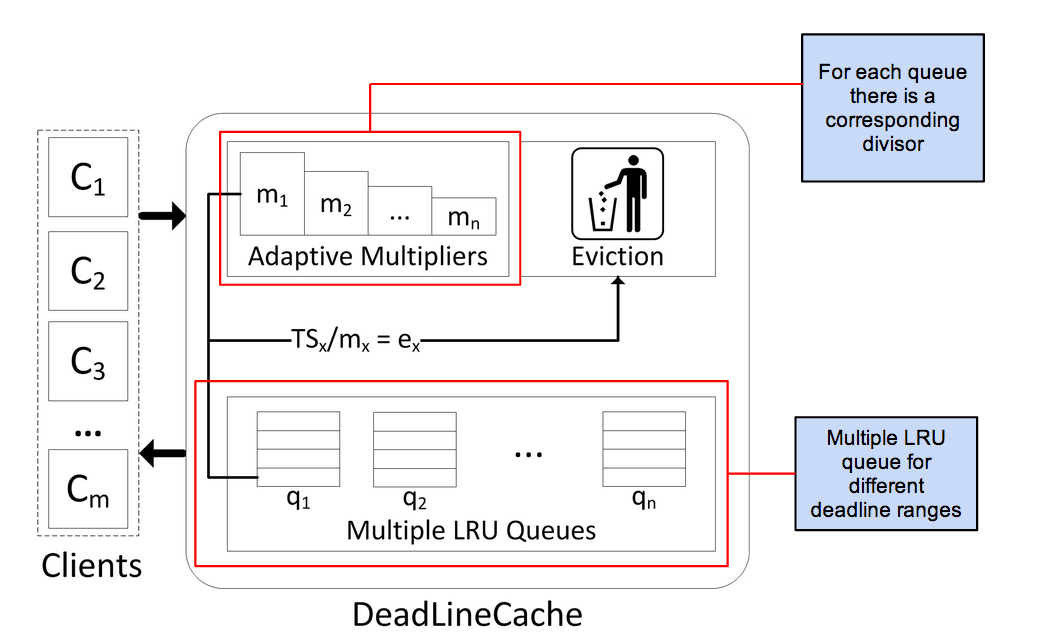
\includegraphics[scale=0.33]{img/DLC_ARC_2.png}}
    \end{center}
  \end{figure}
\end{frame}


%% \begin{frame}
  %% \frametitle{Deadline Cache (DLC) - Components}
  %% \begin{figure}
    %% \begin{center}
      %% \centerline{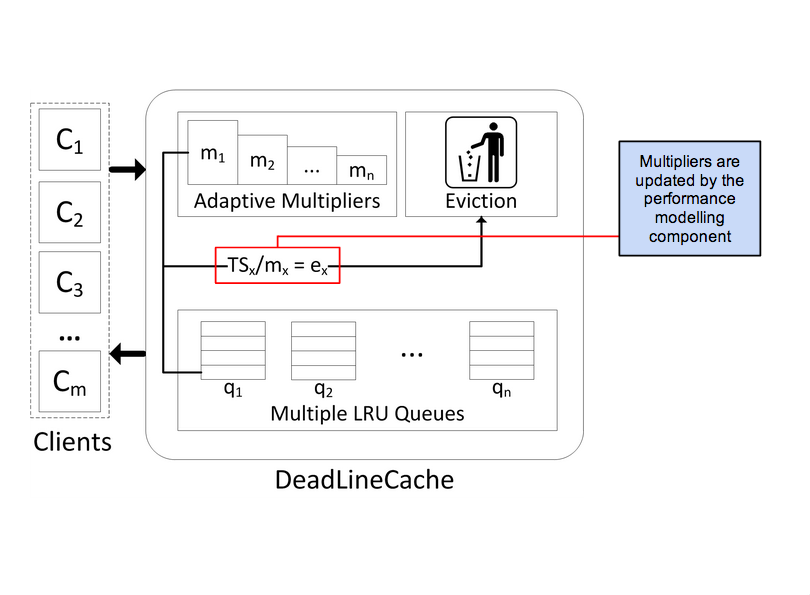
\includegraphics[scale=0.45]{img/DLC_ARC_3.png}}
    %% \end{center}
  %% \end{figure}
%% \end{frame}

\begin{frame}
  \frametitle{DLC - A Cache Eviction Example (1)}
  \begin{figure}
    \begin{center}
      %% \centerline{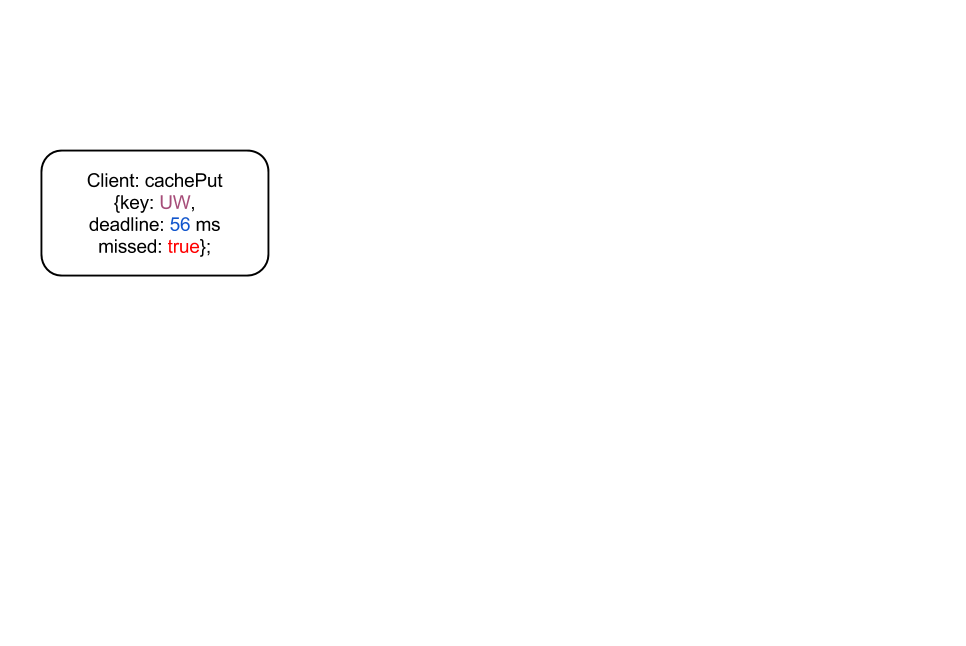
\includegraphics[scale=0.33]{img/DLC_V6_1.png}}
      \centerline{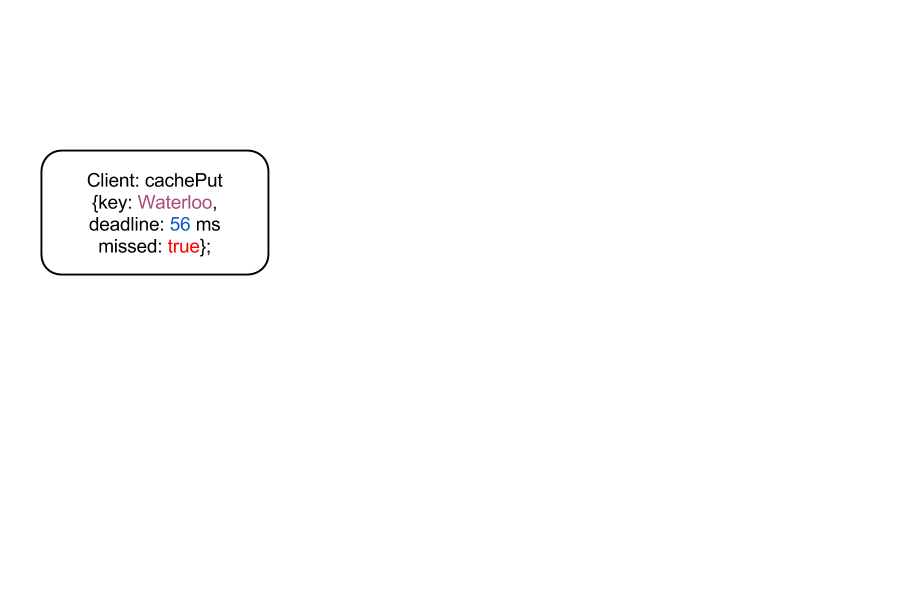
\includegraphics[scale=0.37]{img/DLC_V8_01.png}}
    \end{center}
  \end{figure}
\end{frame}


\begin{frame}
  \frametitle{DLC - A Cache Eviction Example (2)}
  \begin{figure}
    \begin{center}
      %% \centerline{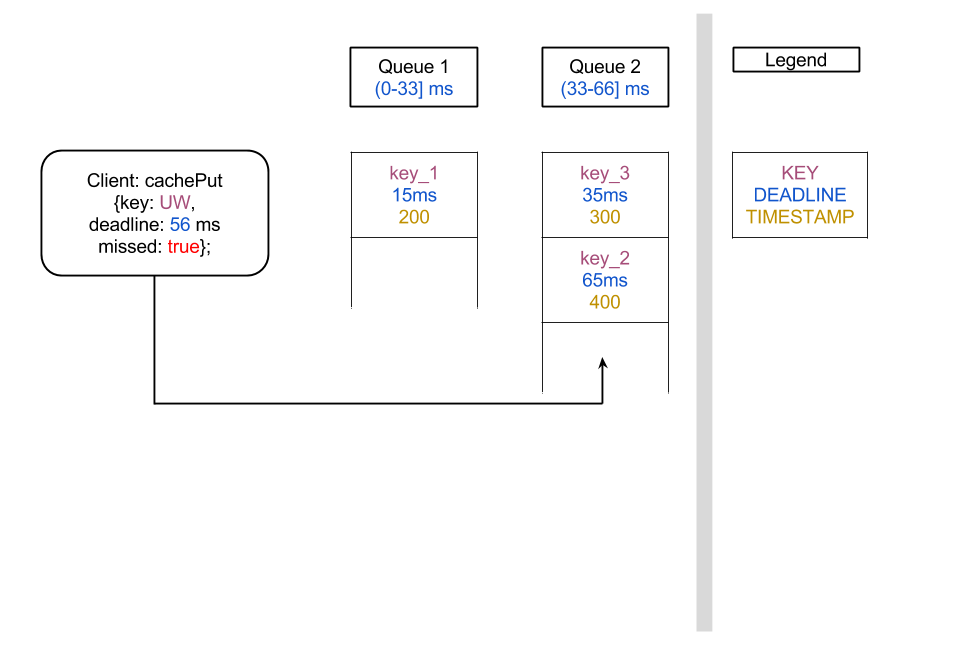
\includegraphics[scale=0.33]{img/DLC_V6_2.png}}
      \centerline{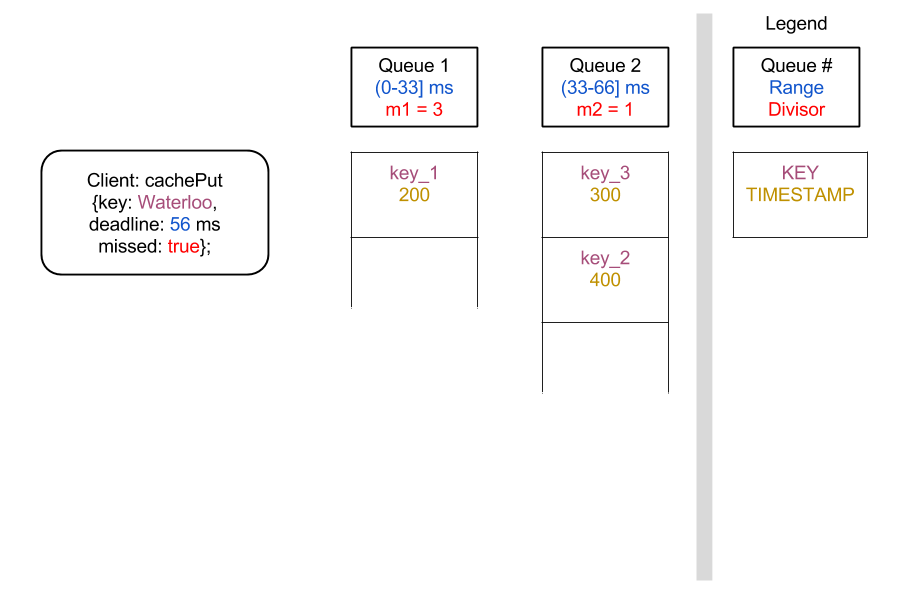
\includegraphics[scale=0.37]{img/DLC_V8_02.png}}
    \end{center}
  \end{figure}
\end{frame}

\begin{frame}
  \frametitle{DLC - A Cache Eviction Example (3)}
  \begin{figure}
    \begin{center}
      %% \centerline{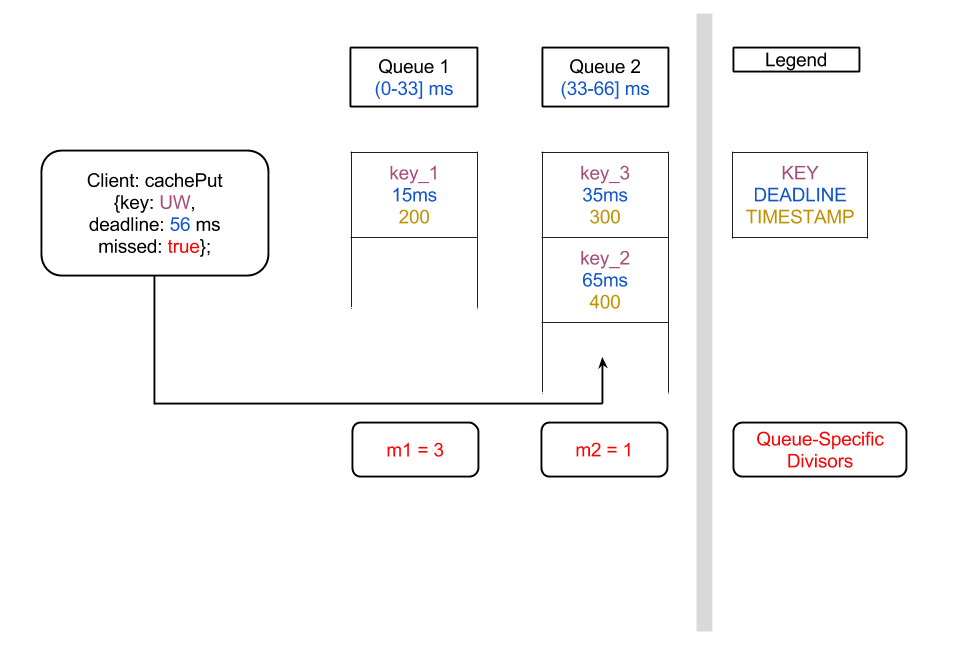
\includegraphics[scale=0.33]{img/DLC_V6_3.png}}
      \centerline{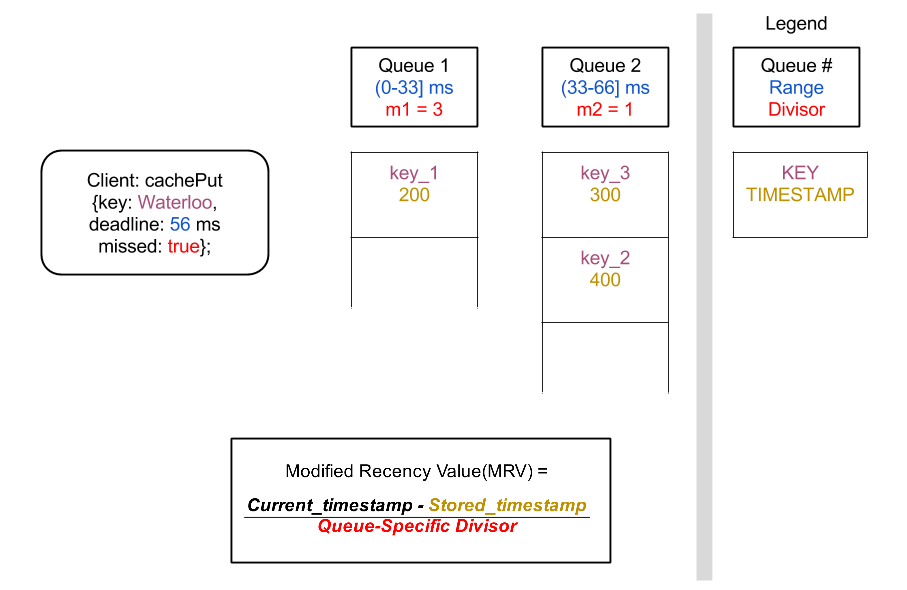
\includegraphics[scale=0.37]{img/DLC_V8_03.png}}
    \end{center}
  \end{figure}
\end{frame}

\begin{frame}
  \frametitle{DLC - A Cache Eviction Example (4)}
  \begin{figure}
    \begin{center}
      %% \centerline{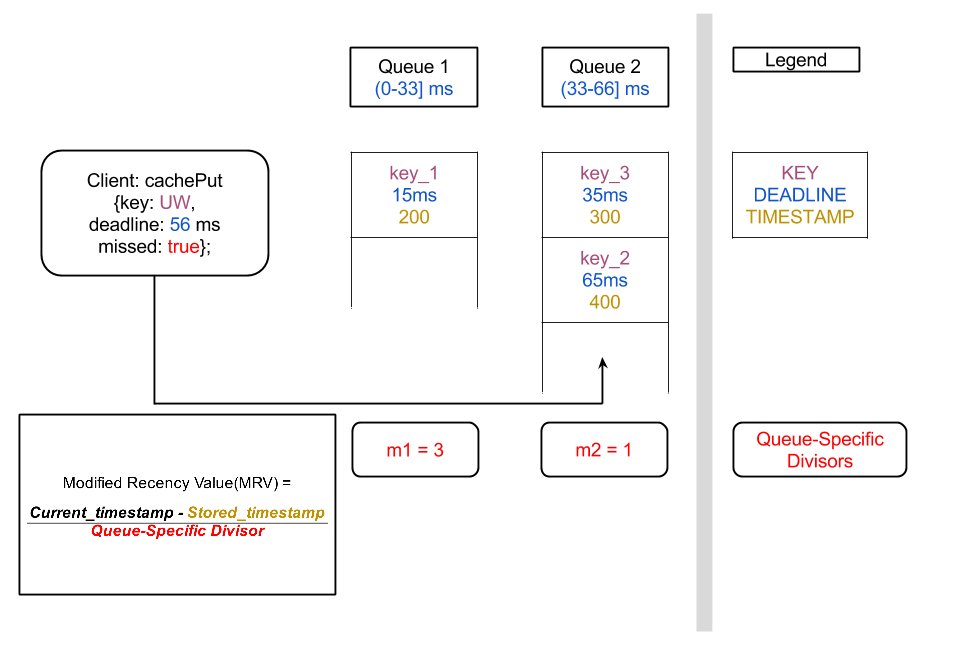
\includegraphics[scale=0.33]{img/DLC_V6_4.png}}
      \centerline{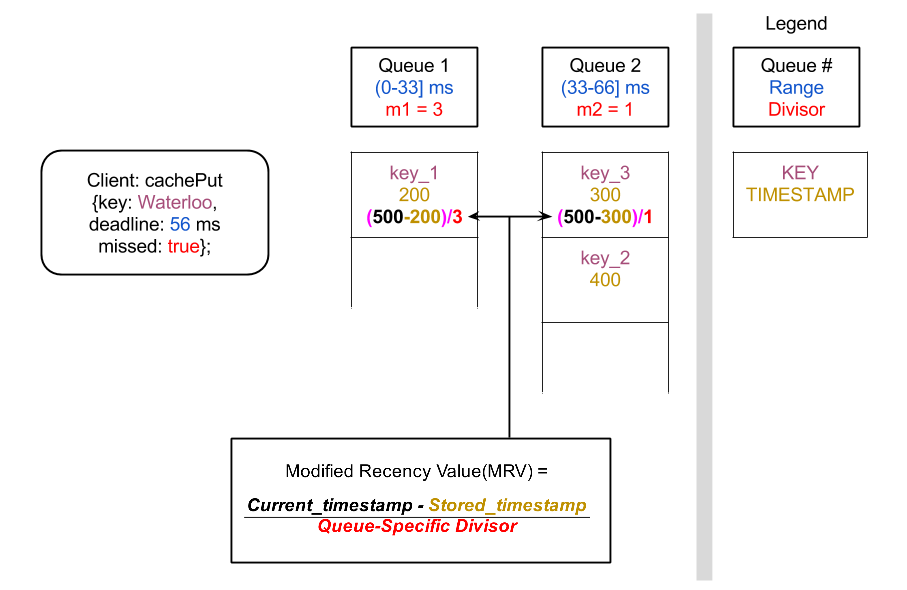
\includegraphics[scale=0.37]{img/DLC_V8_04.png}}
    \end{center}
  \end{figure}
\end{frame}


\begin{frame}
  \frametitle{DLC - A Cache Eviction Example (5)}
  \begin{figure}
    \begin{center}
      %% \centerline{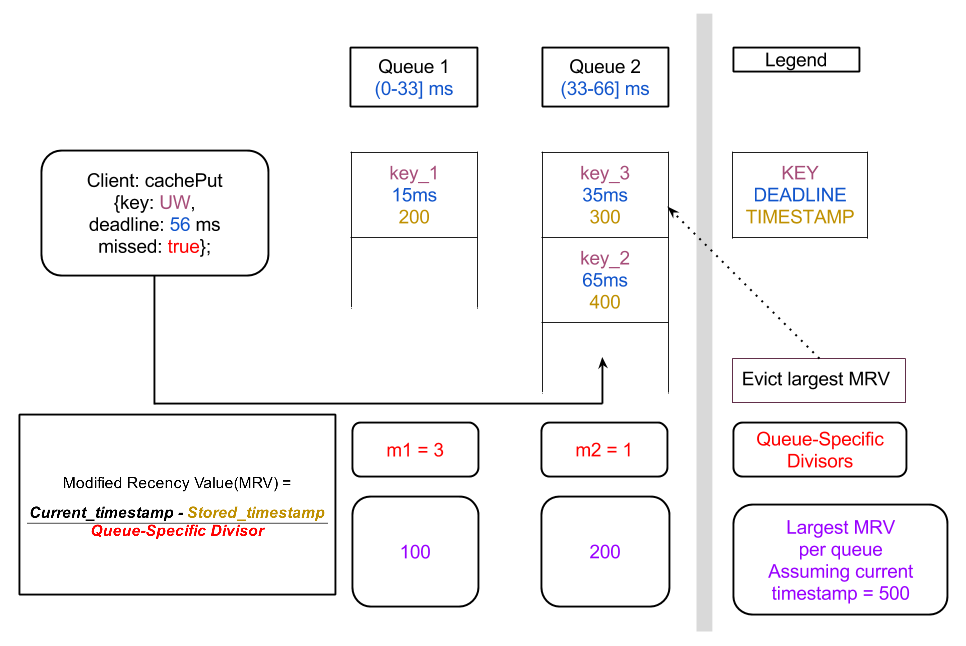
\includegraphics[scale=0.33]{img/DLC_V6_5.png}}
      \centerline{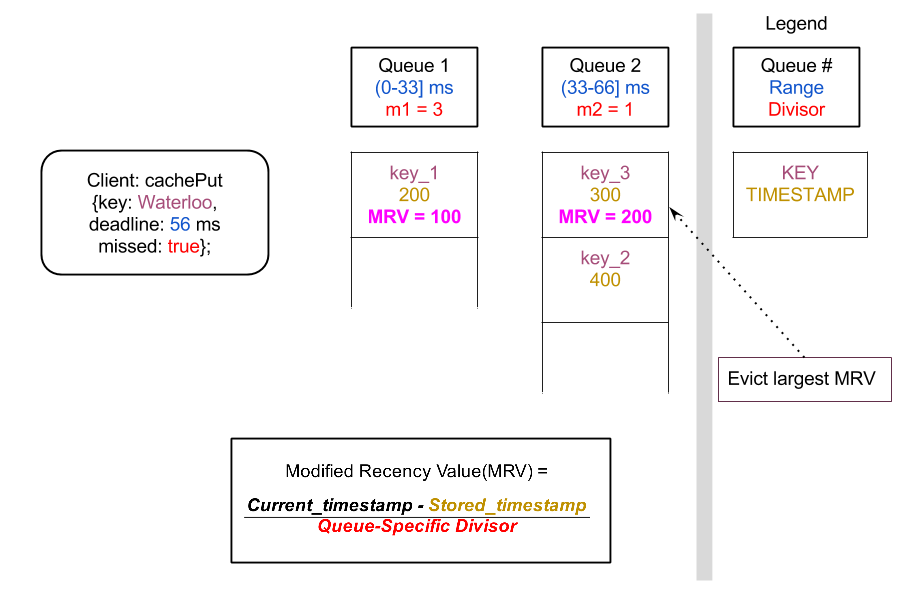
\includegraphics[scale=0.37]{img/DLC_V8_05.png}}
    \end{center}
  \end{figure}
\end{frame}

\begin{frame}
  \frametitle{DLC - A Cache Eviction Example (6)}
  \begin{figure}
    \begin{center}
      %% \centerline{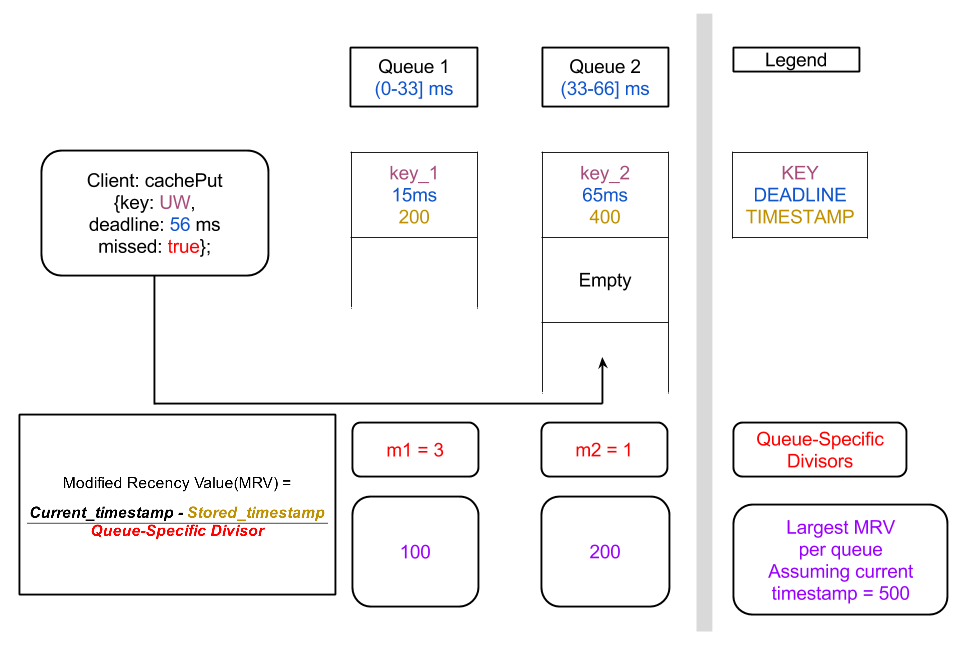
\includegraphics[scale=0.33]{img/DLC_V6_6.png}}
      \centerline{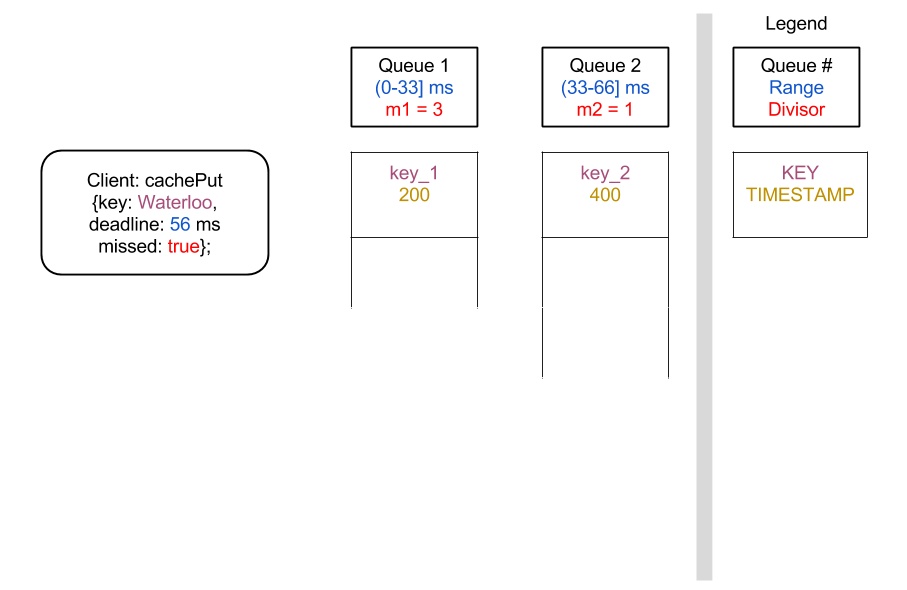
\includegraphics[scale=0.37]{img/DLC_V8_06.png}}
    \end{center}
  \end{figure}
\end{frame}

\begin{frame}
  \frametitle{DLC - A Cache Eviction Example (7)}
  \begin{figure}
    \begin{center}
      %% \centerline{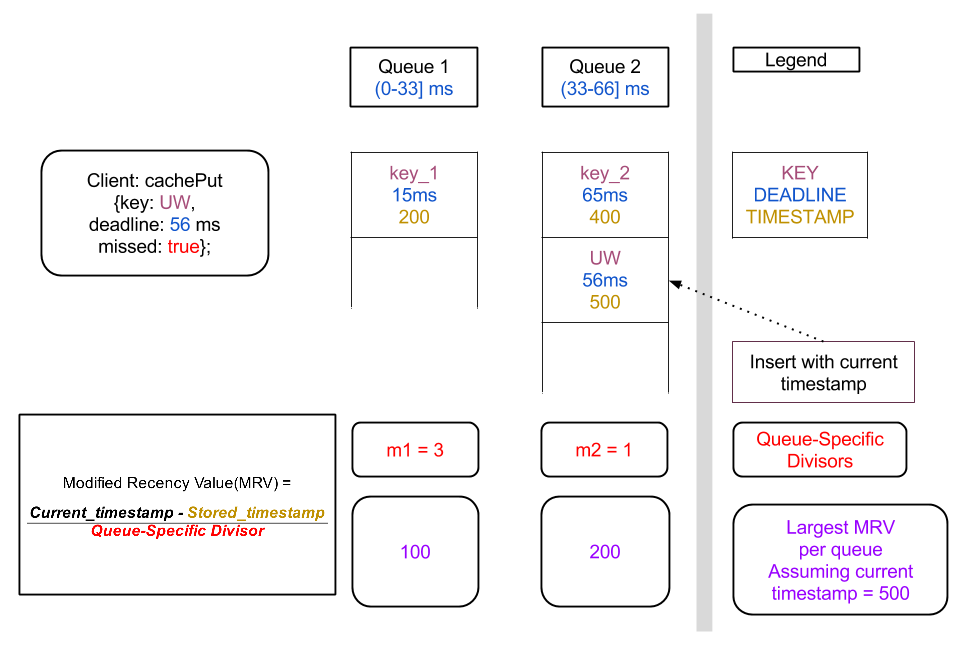
\includegraphics[scale=0.33]{img/DLC_V6_7.png}}
      \centerline{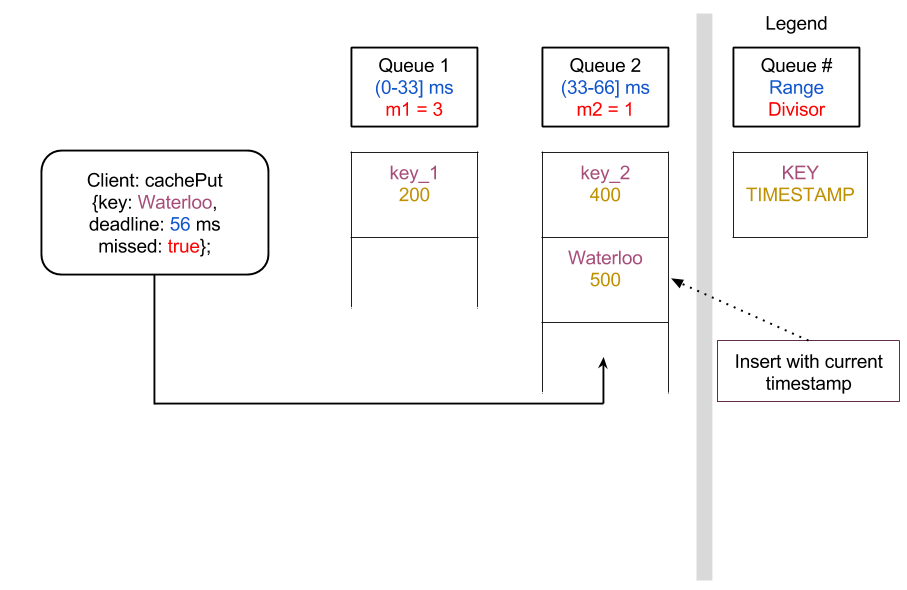
\includegraphics[scale=0.37]{img/DLC_V8_07.png}}
    \end{center}
  \end{figure}
\end{frame}

\begin{frame}
  \frametitle{DLC - A Cache Eviction Example (8)}
  \begin{figure}
    \begin{center}
      %% \centerline{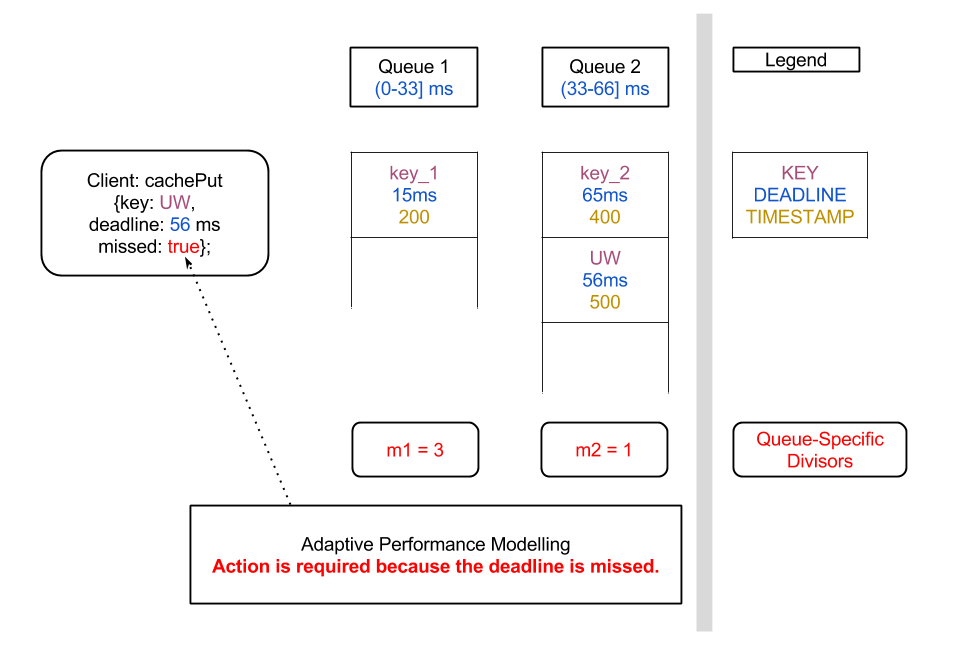
\includegraphics[scale=0.33]{img/DLC_V6_8.png}}
      \centerline{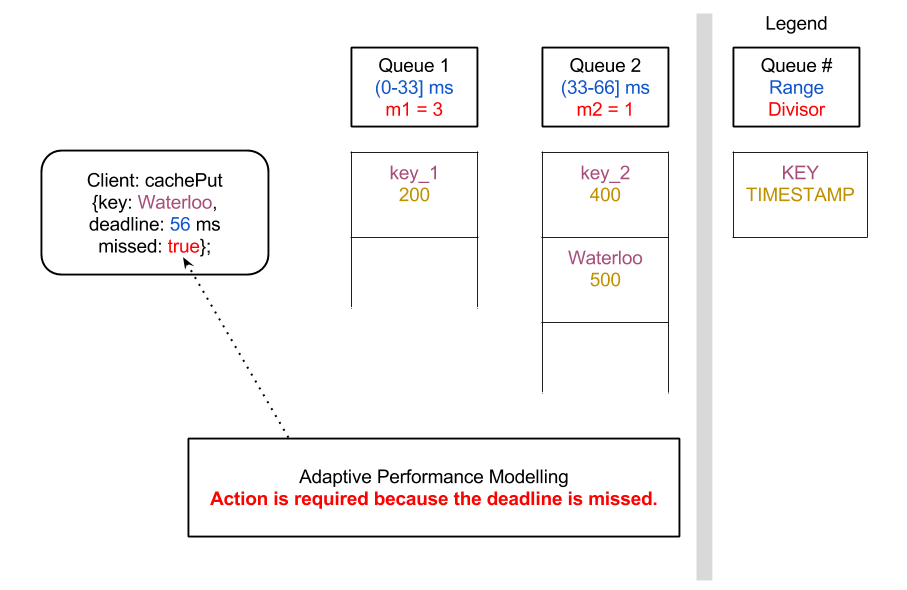
\includegraphics[scale=0.37]{img/DLC_V8_08.png}}
    \end{center}
  \end{figure}
\end{frame}

\begin{frame}
  \frametitle{DLC - A Cache Eviction Example (9)}
  \begin{figure}
    \begin{center}
      %% \centerline{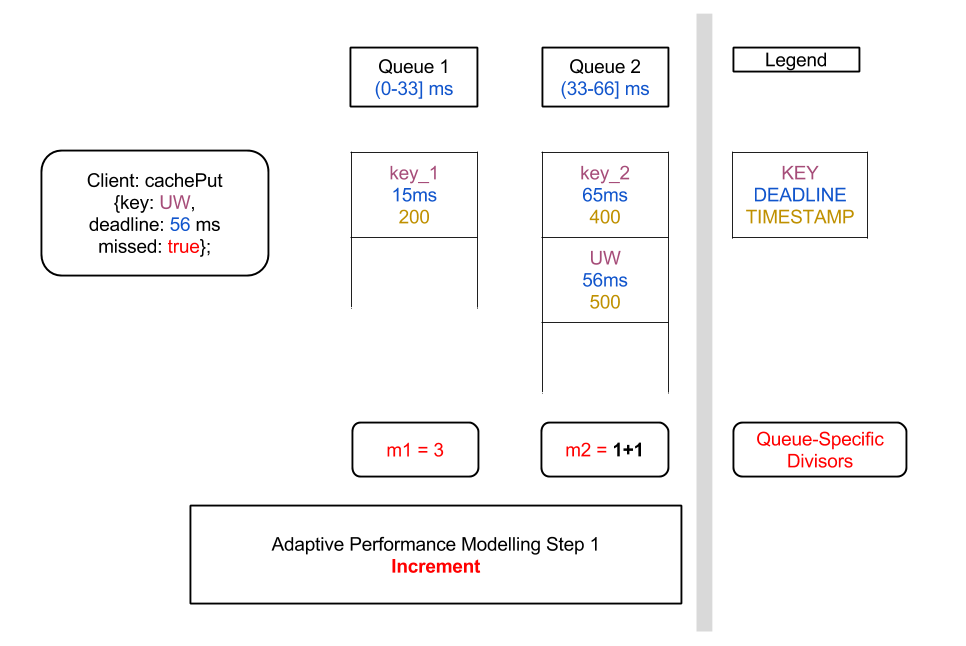
\includegraphics[scale=0.33]{img/DLC_V6_9.png}}
      \centerline{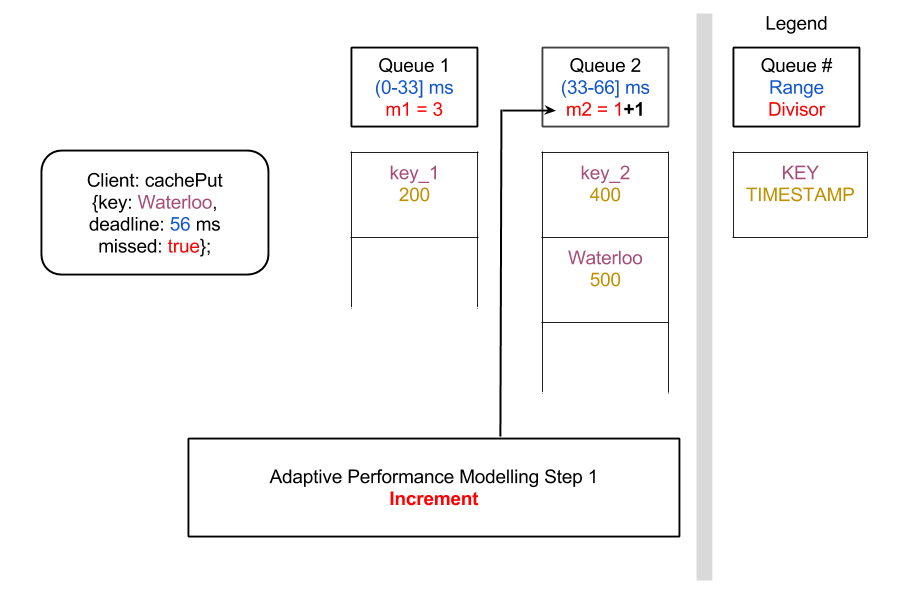
\includegraphics[scale=0.37]{img/DLC_V8_09.png}}
    \end{center}
  \end{figure}
\end{frame}

\begin{frame}
  \frametitle{DLC - A Cache Eviction Example (10)}
  \begin{figure}
    \begin{center}
      %% \centerline{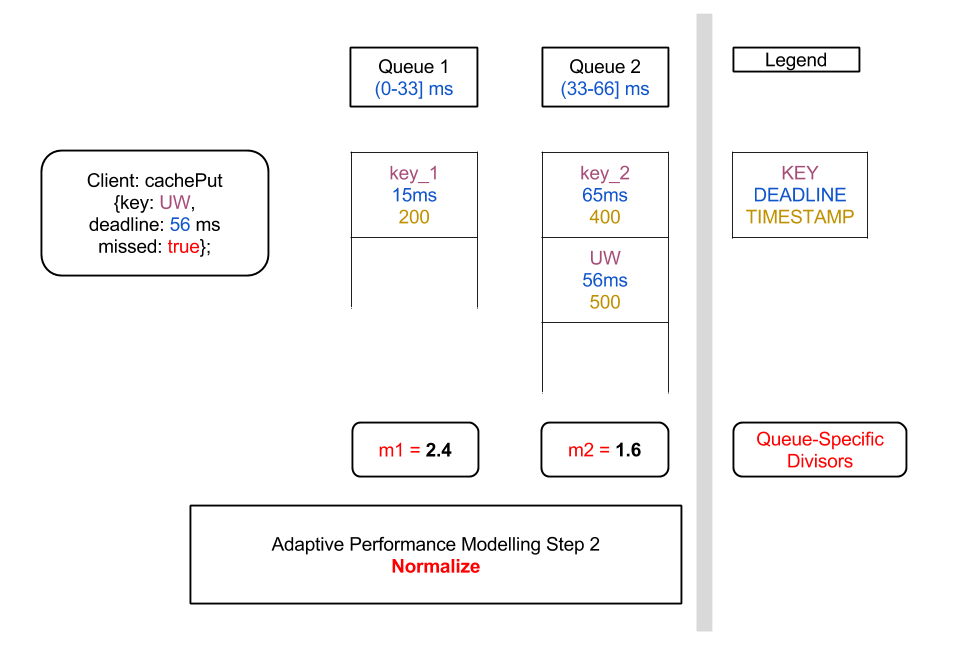
\includegraphics[scale=0.33]{img/DLC_V6_10.png}}
      \centerline{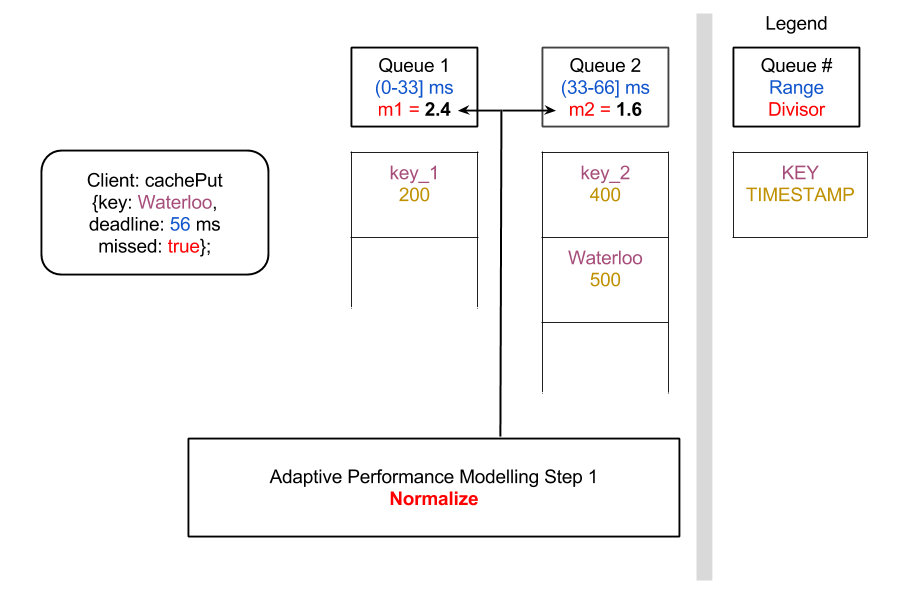
\includegraphics[scale=0.37]{img/DLC_V8_10.png}}
    \end{center}
  \end{figure}
\end{frame}

\begin{frame}
  \frametitle{DLC - Benefits}
  \vspace{-15 mm}
  \begin{itemize}
  \item Multiple LRU queues enable DLC to perform deadline-aware evictions.
    \myv
  \item Adaptive policy considers both the client request rate for each
    deadline range and the underlying system's performance.  \myv

  \item \textbf{DLC} offers adaptive deadline-aware caching.
  \end{itemize}
\end{frame}


%% \begin{frame}
  %% \frametitle{Deadline Scheduler (DLS) High-level Architecture}
  %% \begin{itemize}
  %% \item Scheduler is responsible for controlling access to
    %% data-server.
  %% \end{itemize}
  %% \begin{figure}
    %% \begin{center}
      %% \centerline{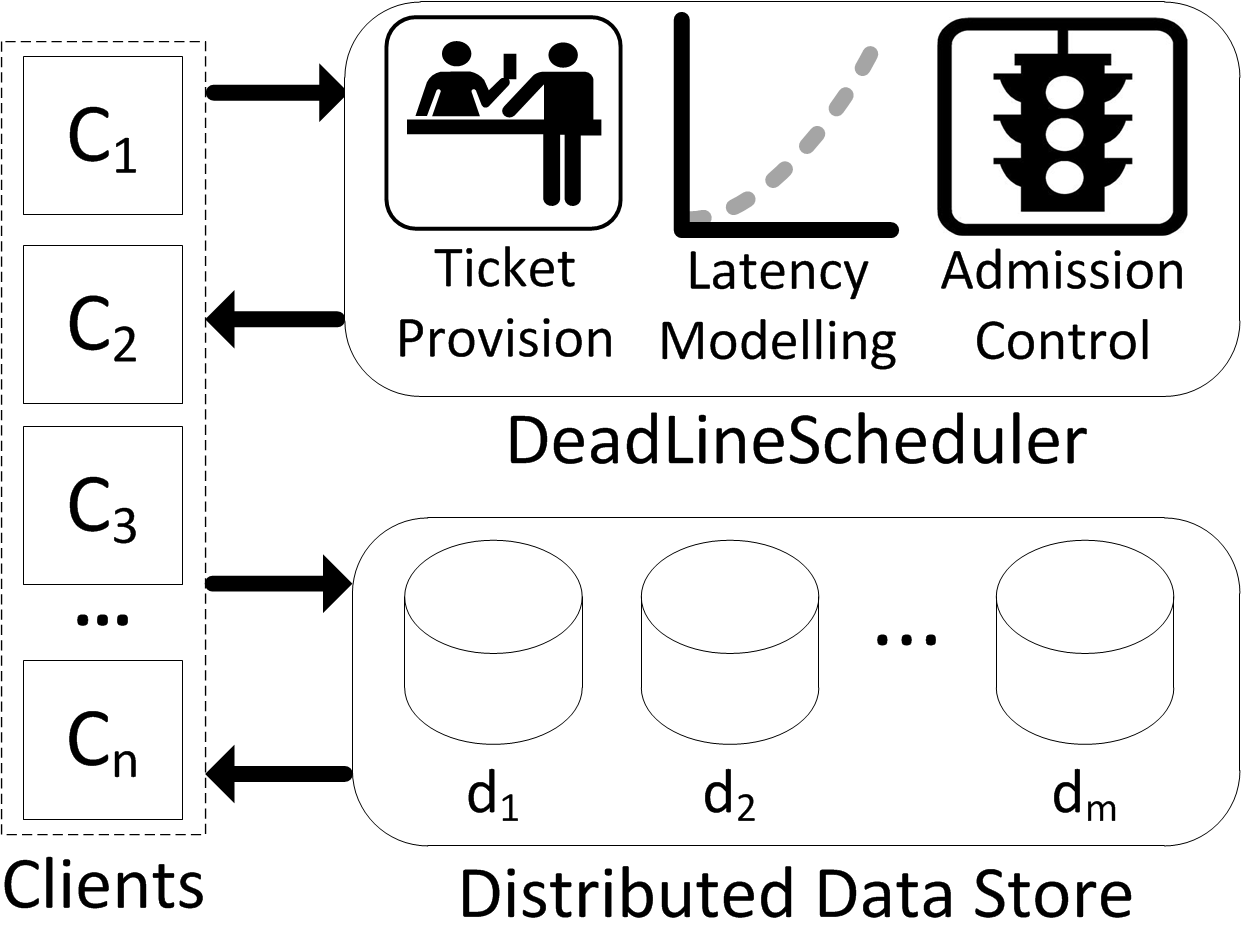
\includegraphics[scale=0.90]{img/DLS.png}}
    %% \end{center}
  %% \end{figure}
%% \end{frame}

\begin{frame}
  \frametitle{Deadline Scheduler (DLS) High-level Architecture \rom{1}}
  \begin{figure}
    \begin{center}
      \centerline{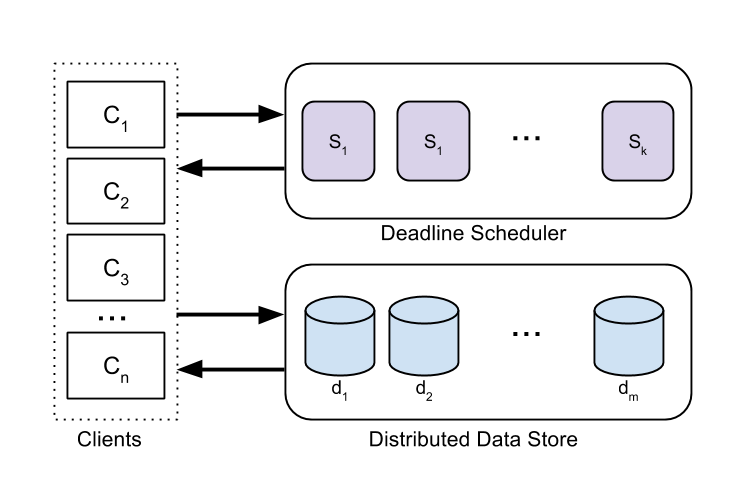
\includegraphics[scale=0.44]{img/DLS_ARCH_1.png}}
    \end{center}
  \end{figure}
\end{frame}
\begin{frame}
  \frametitle{Deadline Scheduler (DLS) High-level Architecture \rom{2}}
  \begin{figure}
    \begin{center}
      \centerline{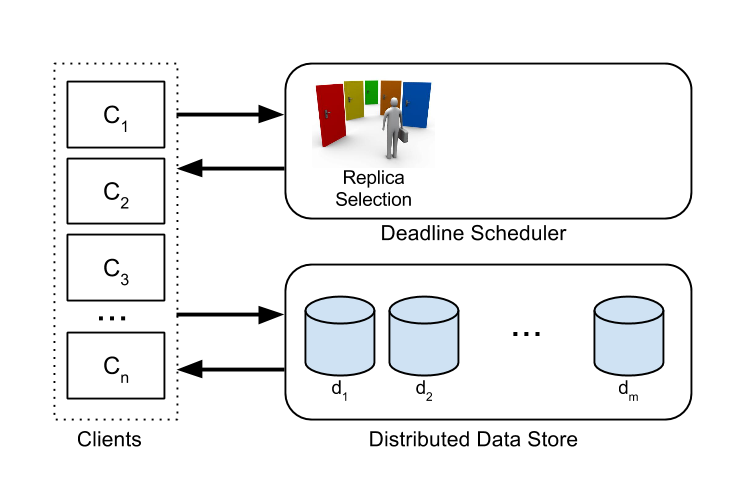
\includegraphics[scale=0.44]{img/DLS_ARCH_2.png}}
    \end{center}
  \end{figure}
\end{frame}
\begin{frame}
  \frametitle{Deadline Scheduler (DLS) High-level Architecture \rom{3}}
  \begin{figure}
    \begin{center}
      \centerline{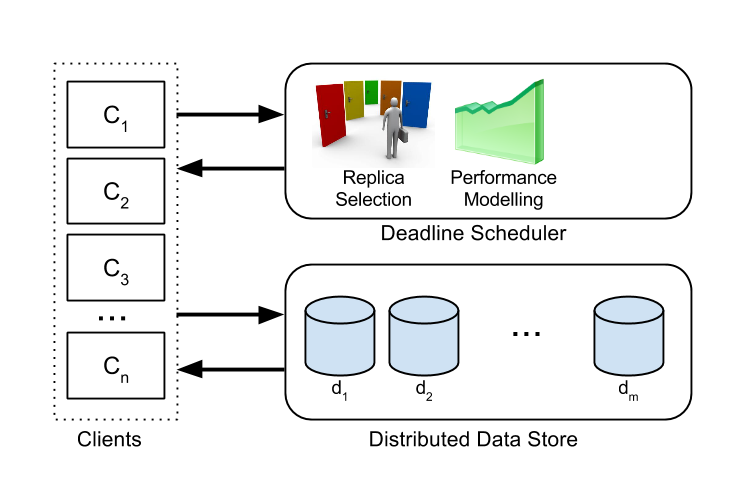
\includegraphics[scale=0.44]{img/DLS_ARCH_3.png}}
    \end{center}
  \end{figure}
\end{frame}
\begin{frame}
  \frametitle{Deadline Scheduler (DLS) High-level Architecture \rom{4}}
  \begin{figure}
    \begin{center}
      \centerline{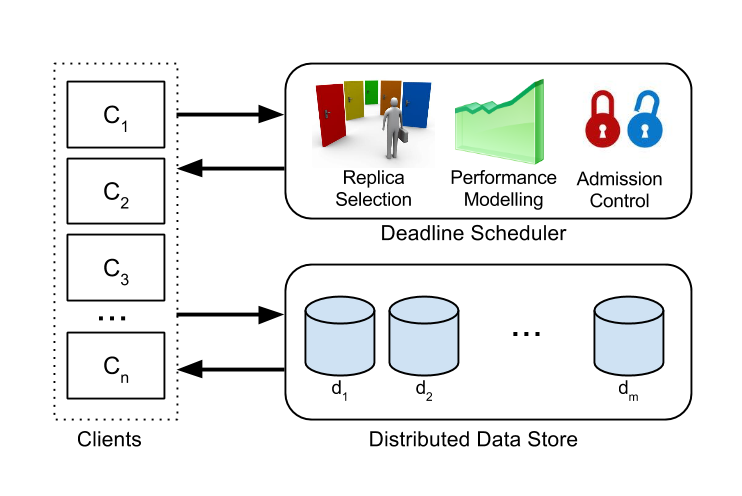
\includegraphics[scale=0.44]{img/DLS_ARCH_4.png}}
    \end{center}
  \end{figure}
\end{frame}





\begin{frame}
  \frametitle{DLS - An Example (1)}
  \begin{itemize}
  \item The client wants to perform a value lookup for the key Waterloo.
  \end{itemize}
  \begin{figure}
    \begin{center}
      \centerline{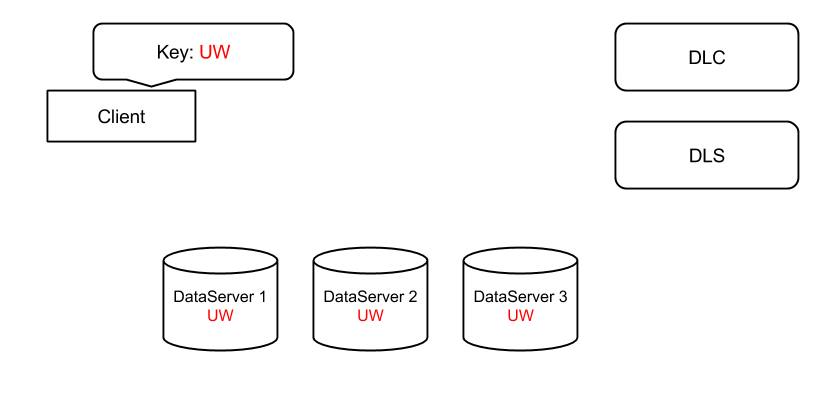
\includegraphics[scale=0.40]{img/DLS_Example01.png}}
    \end{center}
  \end{figure}
\end{frame}

\begin{frame}
  \frametitle{DLS - An Example (2)}
  \begin{itemize}
  \item The client begins by issuing a cache lookup to DLC.
\newline
  \end{itemize}
  \begin{figure}
    \begin{center}
      \centerline{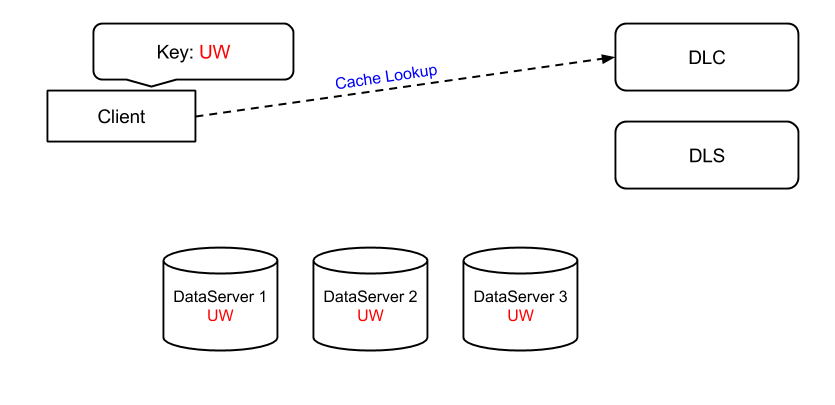
\includegraphics[scale=0.40]{img/DLS_Example02.png}}
    \end{center}
  \end{figure}
\end{frame}

\begin{frame}
  \frametitle{DLS - An Example (3)}
  \begin{itemize}
  \item Issue two \textit{get ticket} requests concurrently.
\newline
  \end{itemize}
  \begin{figure}
    \begin{center}
      \centerline{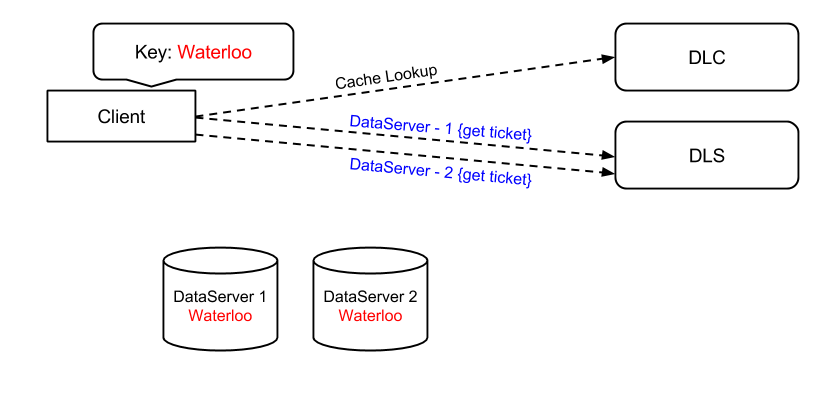
\includegraphics[scale=0.40]{img/DLS_Example03.png}}
    \end{center}
  \end{figure}
\end{frame}

\begin{frame}
  \frametitle{DLS - An Example (4)}
  \begin{itemize}
  \item If the item is not in the cache, the client waits for DLS to
    return the tickets.
    %% \vspace{-0.1 mm}
  \end{itemize}
  \begin{figure}
    \begin{center}
      \centerline{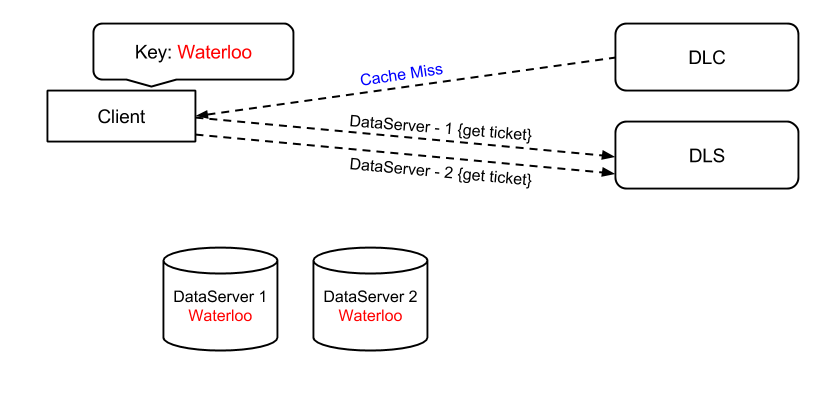
\includegraphics[scale=0.40]{img/DLS_Example04.png}}
    \end{center}
  \end{figure}
\end{frame}


\begin{frame}
  \frametitle{DLS - An Example (5)}
  \begin{itemize}
  \item Returned tickets contain extra information to help the client to make
    an informed decision.
  \end{itemize}
  \begin{figure}
    \begin{center}
      \centerline{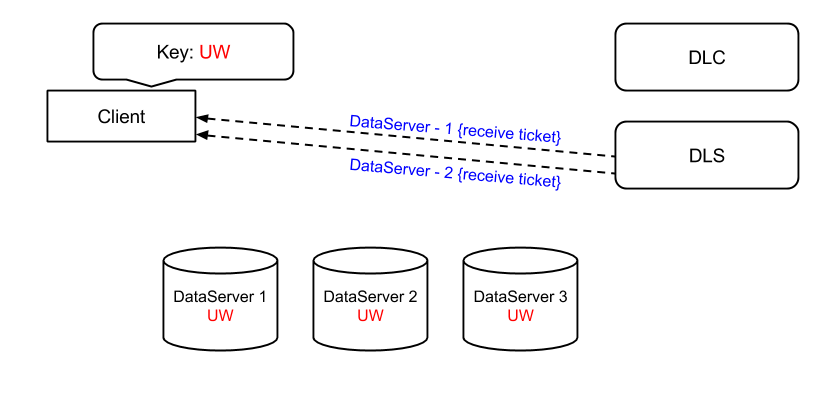
\includegraphics[scale=0.40]{img/DLS_Example05.png}}
    \end{center}
  \end{figure}
\end{frame}

\begin{frame}
  \frametitle{DLS - An Example (6)}
  \begin{itemize}
  \item The client makes a call to the selected DLS and waits for
    its turn to access the data server.
  \end{itemize}
  \begin{figure}
    \begin{center}
      \centerline{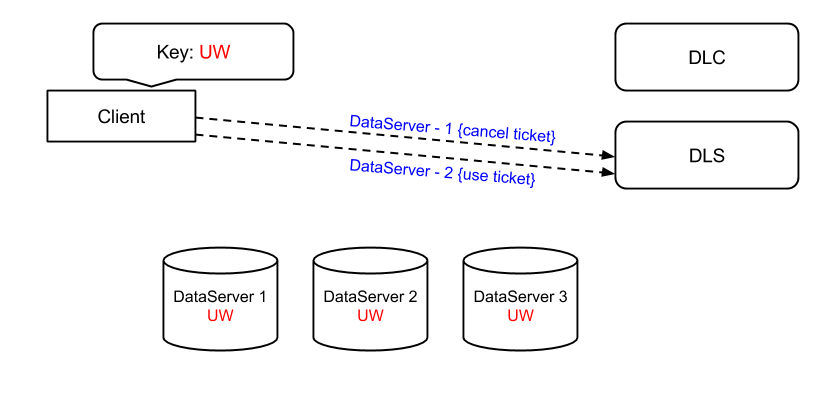
\includegraphics[scale=0.40]{img/DLS_Example06.png}}
    \end{center}
  \end{figure}
\end{frame}

\begin{frame}
  \frametitle{DLS - An Example (7)}
  \begin{itemize}
  %% \item Let's look at how requests are scheduled inside scheduler's pending
    %% queue.
  \item Snapshot of scheduler's pending queue.
    \newline
    \newline
  \end{itemize}
  \vspace{-5 mm}
  \begin{figure}
    \begin{center}
      \centerline{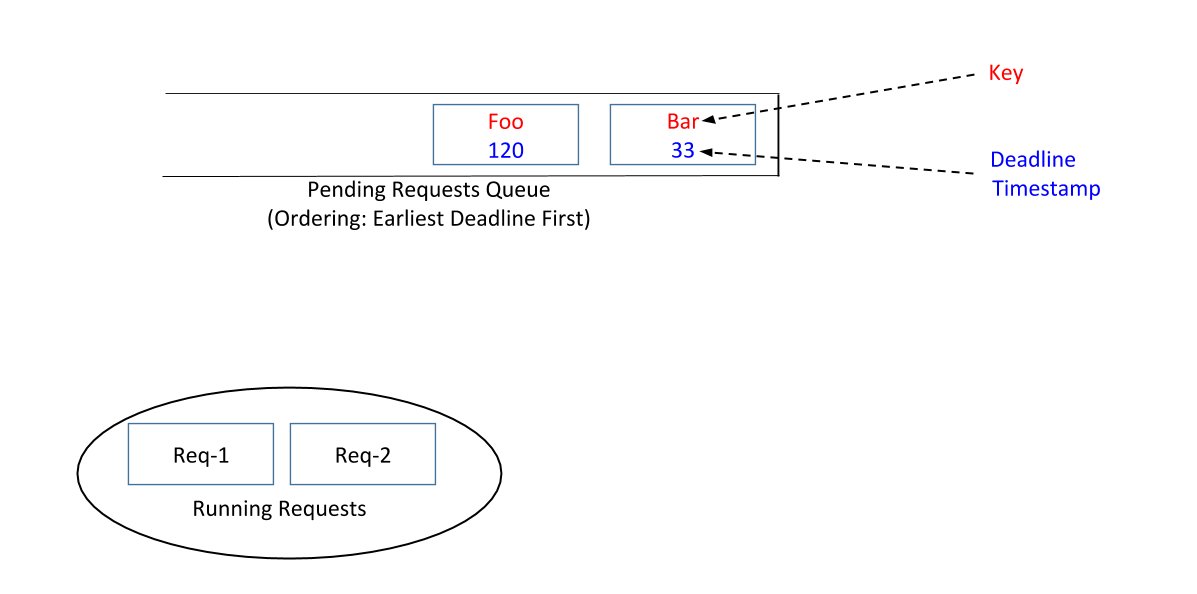
\includegraphics[scale=0.33]{img/DLS_Example_ZOOM_1.png}}
    \end{center}
  \end{figure}
\end{frame}

\begin{frame}
  \frametitle{DLS - An Example (8)}
  \begin{itemize}
  \item The new item is inserted according to earliest deadline first ordering.
    \newline
  \end{itemize}
  \vspace{-5 mm}
  \begin{figure}
    \begin{center}
      \centerline{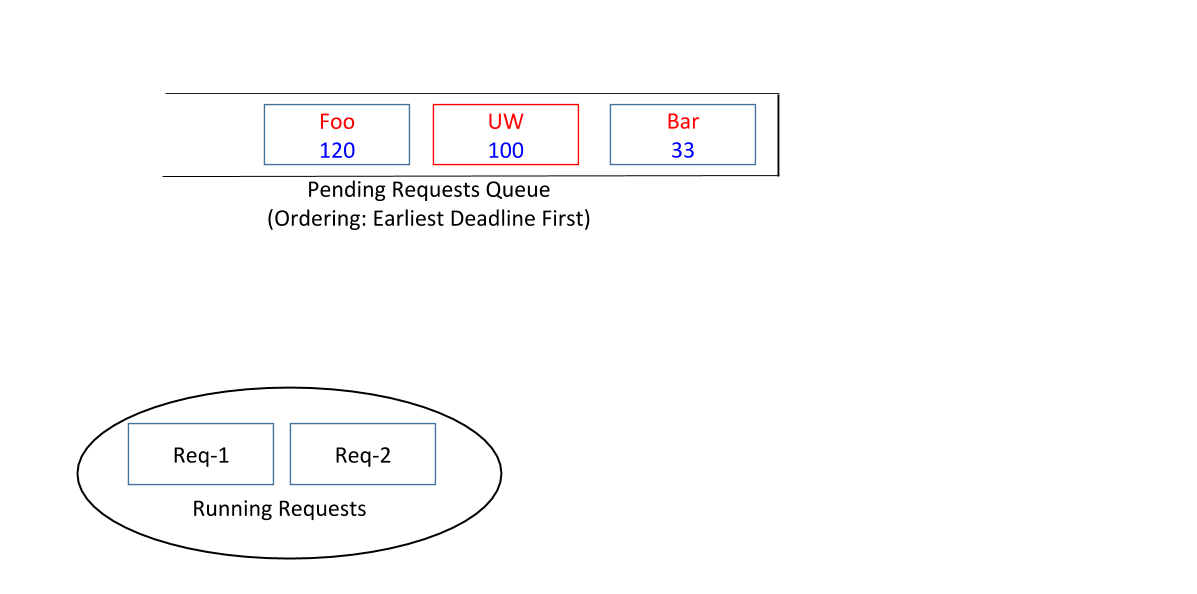
\includegraphics[scale=0.33]{img/DLS_Example_ZOOM_2.png}}
    \end{center}
  \end{figure}
\end{frame}


\begin{frame}
  \frametitle{DLS - An Example (9)}
  \begin{itemize}
  \item Let's assume one of the running requests just completed.
    \newline
    \newline
  \end{itemize}
  \vspace{-5 mm}
  \begin{figure}
    \begin{center}
      \centerline{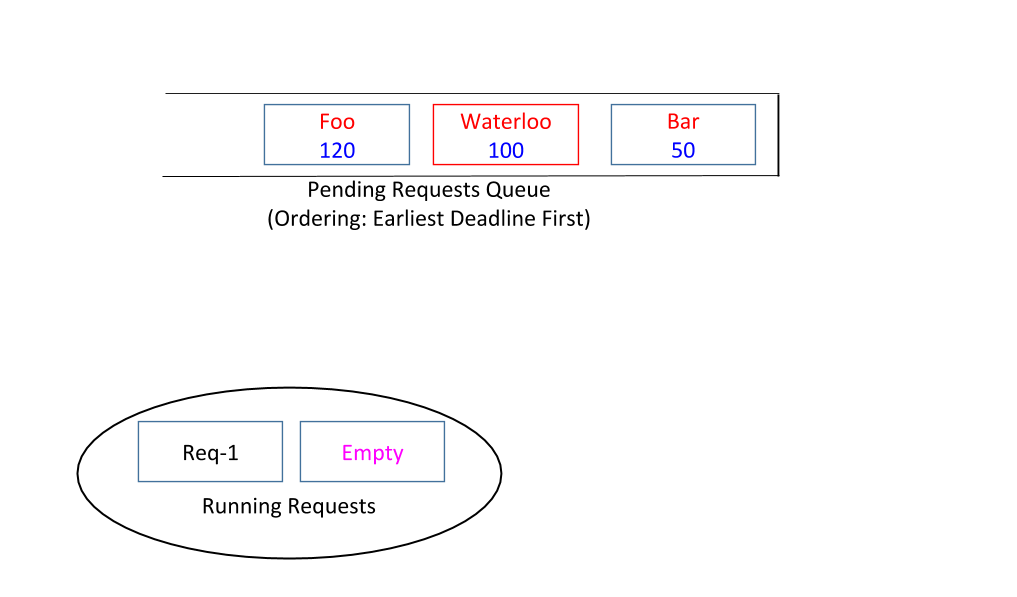
\includegraphics[scale=0.33]{img/DLS_Example_ZOOM_3.png}}
    \end{center}
  \end{figure}
\end{frame}


\begin{frame}
  \frametitle{DLS - An Example (10)}
  \begin{itemize}
  \item If the request deadline can be met, it will take one of the empty slots
    inside the running request pool.
    \newline
  \end{itemize}
  \vspace{-5 mm}
  \begin{figure}
    \begin{center}
      \centerline{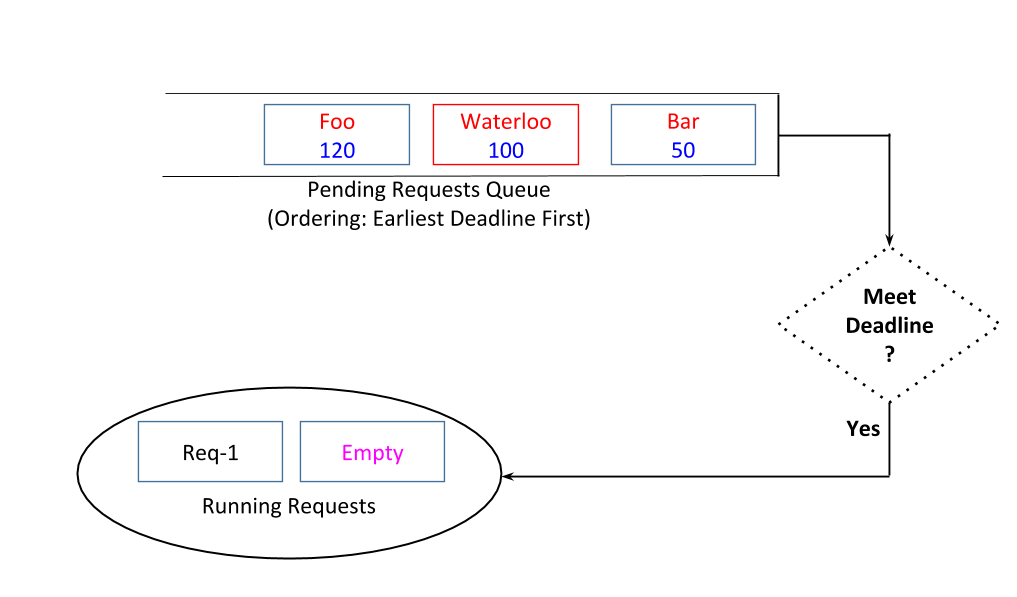
\includegraphics[scale=0.33]{img/DLS_Example_ZOOM_4.png}}
    \end{center}
  \end{figure}
\end{frame}



\begin{frame}
  \frametitle{DLS - An Example (11)}
  \begin{itemize}
  \item If request deadline cannot be met, DLS may increase the request's
    deadline and insert the request back into the queue.
    \newline
  \end{itemize}
  \vspace{-5 mm}
  \begin{figure}
    \begin{center}
      \centerline{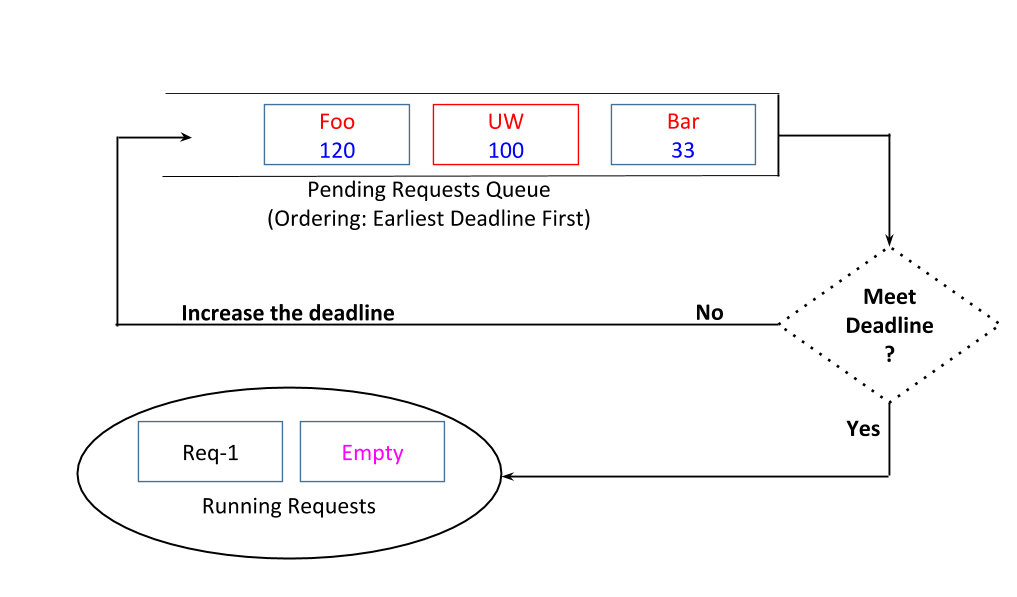
\includegraphics[scale=0.33]{img/DLS_Example_ZOOM_5.png}}
    \end{center}
  \end{figure}
\end{frame}


\begin{frame}
  \frametitle{DLS - An Example (12)}
  \begin{itemize}
  \item The push-back can happen at most once to prevent starvation.
    \newline
    \newline
  \end{itemize}
  \vspace{-5 mm}
  \begin{figure}
    \begin{center}
      \centerline{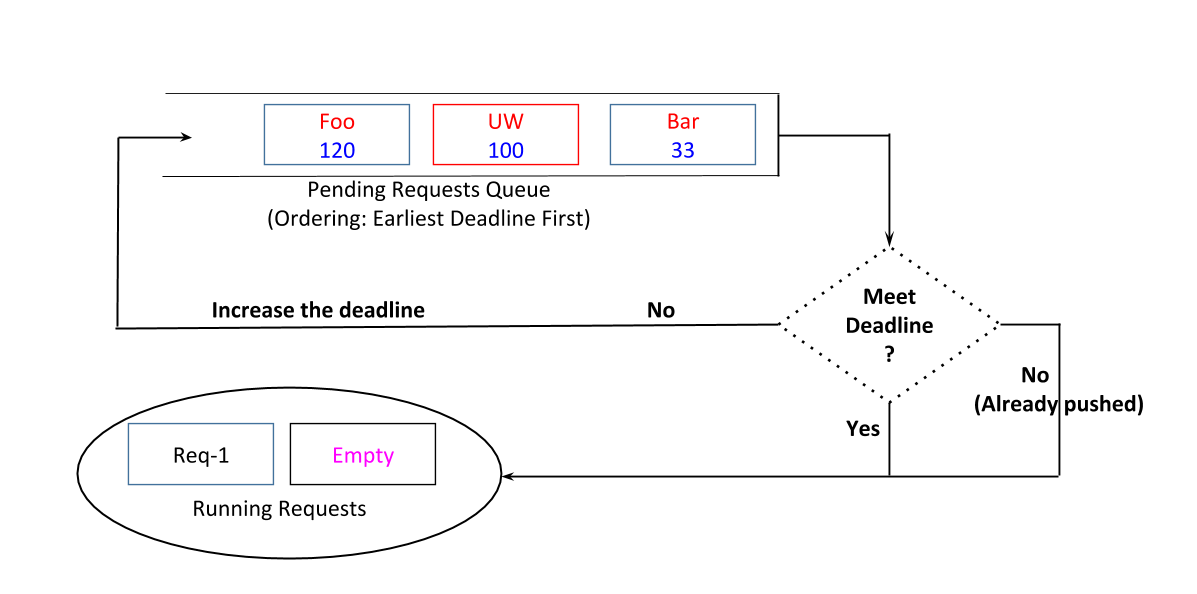
\includegraphics[scale=0.33]{img/DLS_Example_ZOOM_6.png}}
    \end{center}
  \end{figure}
\end{frame}

\begin{frame}
  \frametitle{DLS - An Example (13)}
  \begin{itemize}
  \item DLS informs the client that it can access the data server.
\newline
  \end{itemize}
  \begin{figure}
    \begin{center}
      \centerline{\includegraphics[scale=0.40]{img/DLS_Example07.png}}
    \end{center}
  \end{figure}
\end{frame}

\begin{frame}
  \frametitle{DLS - An Example (14)}
  \begin{itemize}
  \item The client issues the read request to the data server.
\newline
  \end{itemize}
  \begin{figure}
    \begin{center}
      \centerline{\includegraphics[scale=0.40]{img/DLS_Example08.png}}
    \end{center}
  \end{figure}
\end{frame}

\begin{frame}
  \frametitle{DLS - An Example (15)}
  \begin{itemize}
  \item After receiving the response, the client reports
    the execution time and concurrently inserts the data into the cache.
  \end{itemize}
  \vspace{-0.9 mm}
  \begin{figure}
    \begin{center}
      \centerline{\includegraphics[scale=0.40]{img/DLS_Example09.png}}
    \end{center}
  \end{figure}
\end{frame}

\begin{frame}
  \frametitle{DLS - Benefits}
  % xcuiTODO: Make summary smaller June 20th
  \begin{itemize}
  %% \item A load-balancing system that directs each client to the server that is
    %% most likely to meet each request's deadline.
  \item Deadline-aware load-balancing.
    \myv
  %% \item A variant of earliest deadline first scheduling that limits the impact
    %% of deadline violations on other requests.
  \item A variant of earliest deadline first scheduling.
    \myv
  %% \item A tunable admission control system that bounds the percentage of
    %% requests missing their deadlines.
  \item Tunable admission control system.
  \end{itemize}
\end{frame}

%% \begin{frame}
  %% \frametitle{Goals of the Evaluation}
  %% \begin{itemize}
  %% \item Comparison of the two caching systems.
    %% \begin{itemize}
    %% \item Deadline Cache
    %% \item Memcached
    %% \end{itemize}
  %% \item Effectiveness of MicroFuge.
    %% \begin{itemize}
    %% \item Caching Layer
    %% \item Scheduling layer
    %% \item Admission control
    %% \end{itemize}
  %% \end{itemize}
%% \end{frame}


\begin{frame}
  \frametitle{Experimental Setup - The Cluster}
  \begin{itemize}
  \item Twenty-node test cluster on AWS. Each cluster node is an m1.medium
    EC2 instance.
  \end{itemize}
  \begin{figure}
    \begin{center}
      \centerline{\includegraphics[scale=0.25]{img/Experimental_Setup.png}}
    \end{center}
  \end{figure}
\end{frame}

\begin{frame}
  \frametitle{Experimental Setup - Details}
  \begin{itemize}
  \item DataServer - Simple key-value store that uses leveldb.
  \item We use a replication factor of 3.
  \item Benchmarking System - Modified version of Yahoo! Cloud Serving
    Benchmark (YCSB).
    \begin{itemize}
    \item Assign deadlines to each key.\\
      %% \begin{center}
      \begin{tabular}{| l | c |}
        \hline
        Range & Percentage \\ \hline
        10-30ms & 20\% \\ \hline
        30-100ms & 30\% \\ \hline
        100-1000ms & 50\% \\ \hline
      \end{tabular}
      %% \end{center}
    \end{itemize}
  \item Data Set - 80 million records, 86.4 GB in size.
  \item Cache - Total capacity of 19.2GB.
  \end{itemize}
  % NOTES: We selected one range of deadlines which looked reasonable to us.
\end{frame}


\begin{frame}
  \frametitle{Deadline-Aware Caching - \textbf{DLC}}
  \begin{figure}[t]
    \begin{center}
      \centerline{\includegraphics[scale=0.5]{img/EC2/EC2_CS_MM/cache_48.png}}
      \caption{Cache hit rate for 192 concurrent clients with DLC and Memcached.}
      \label{fig:cache_192_cs_mm}
    \end{center}
  \end{figure}
\end{frame}

\begin{frame}
  \frametitle{Deadline-Aware Caching - \textbf{Full MicroFuge}}
  \begin{figure}[t]
    \begin{center}
      \centerline{\includegraphics[scale=0.5]{img/EC2/EC2_SH_MM/cache_48.png}}
      \caption{Cache hit rate for 192 concurrent clients with DLC + DLS and Memcached.}
      \label{fig:cache_192_sh_mm}
    \end{center}
  \end{figure}
\end{frame}

\begin{frame}
  \frametitle{Deadline Miss Rate - \textbf{DLC}}
  \begin{figure}[t]
    \begin{center}
      \centerline{\includegraphics[scale=0.5]{img/EC2/EC2_CS_MM/miss_48.png}}
      \caption{Deadline miss rate for 192 concurrent clients with DLC and Memcached.}
      \label{fig:miss_192_cs_mm}
    \end{center}
  \end{figure}
\end{frame}


\begin{frame}
  \frametitle{Deadline Miss Rate - \textbf{Full MicroFuge}}
  \begin{figure}[t]
    \begin{center}
      \centerline{\includegraphics[scale=0.5]{img/EC2/EC2_SH_MM/miss_48.png}}
      \caption{Deadline miss rate for 192 concurrent clients with DLC + DLS and Memcached.}
      \label{fig:miss_192_sh_mm}
    \end{center}
  \end{figure}
\end{frame}


\begin{frame}
  \frametitle{Conclusion}
  \begin{itemize}
  \item Predictable performance is necessary in multi-tenant environments.
    \myv
  \item MicroFuge tackles the performance isolation problem with its
    deadline-aware caching and scheduling middleware.
    \myv
  \item MicroFuge reduces deadline miss rate from 17.5\% to 7.7\% and it can be
    as low as 4.7\% if we turn on the admission control.
  \end{itemize}
\end{frame}

\begin{frame}
  \centerline{Thank You.}
\end{frame}

\begin{frame}
  \frametitle{DLS - Admission Control}
  \begin{itemize}
  \item Bound the fraction of requests that miss their deadlines.
  \item Requests are rejected in two situations.
    \begin{itemize}
    \item The request will be miss its own deadline.
    \item The new request will cause already accepted requests to miss their deadlines.
    \end{itemize}
  \item Provides a system parameter $\beta$ as a knob to control the percentage
    of deadline misses.
  \end{itemize}
\end{frame}

\begin{frame}
  \frametitle{Experimental Results - Deadline Miss with Admission Control}
  \begin{figure}[t]
    \begin{center}
      \centerline{\includegraphics[scale=0.5]{img/EC2/EC2_AC_MM/miss_48.png}}
      \caption{Deadline miss rate for 192 concurrent clients with DLC + DLS + AC and Memcached.}
      \label{fig:miss_192_ac_mm}
    \end{center}
  \end{figure}
\end{frame}

\begin{frame}
  \frametitle{Experimental Results - Tunable Admission Control}
  \begin{figure}[t]
    \begin{center}
      \centerline{\includegraphics[scale=0.5]{img/EC2/Varying_ac/varying_acPerc_192.png}}
      \caption{Deadline miss vs. rejection rates with respect to various values of
        system parameter $\beta$ for 192 clients.}
      \label{fig:varying_ac}
    \end{center}
  \end{figure}
\end{frame}

\begin{frame}
  \frametitle{MicroFuge at a Glance}
  \begin{itemize}
  \item Middleware for popular key-value storage.
    \myv
  \item A modified version of the CRUD operation interface.
    %% \centering
  \end{itemize}
  \begin{figure}
    %% \begin{flushleft}
    \vspace{-5 mm}
    \includegraphics[scale=0.15]{img/MicroFuge_protocol.png}
    \caption{MicroFuge \textit{read} operation interface.}
    %% \end{flushleft}
  \end{figure}
\end{frame}

\end{document}
